\documentclass[11pt]{article}

% Compact anonymous ML-conference style.
\usepackage[margin=1in]{geometry}
\usepackage{times}
\usepackage{amsmath,amssymb}
\usepackage{booktabs}
\usepackage{graphicx}
\usepackage{multirow}
\usepackage[numbers]{natbib}
\usepackage{hyperref}
\usepackage{xcolor}
\usepackage[most]{tcolorbox}
\usepackage{enumitem}
\usepackage{caption}
\hypersetup{hidelinks}

\newcommand{\todo}[1]{\textcolor{red}{\textbf{[TODO: #1]}}}
\newcommand{\method}[1]{\texttt{#1}}
\newcommand{\sac}{\textsc{SAC}}
\newcommand{\asr}{\mathrm{ASR}}
\setlength{\emergencystretch}{2em}

\twocolumn
\setlength{\columnsep}{0.6cm}

\title{Security-Aware Selective Compression for Mitigating LoRA Backdoors in Large Language Models}

\author{Anonymous}

\date{}

\begin{document}
\maketitle

% Result source: /mnt/disk/xlz/SAC/single/docs/results_summary.md
\begin{abstract}
Parameter-efficient adapters make large language models easy to specialize and distribute, but they also create a compact attack surface: a malicious LoRA adapter can implant backdoor behavior while leaving the base model unchanged.
Post-training compression is a natural deployment-time intervention for such adapters, yet existing compression objectives are not designed to remove malicious behaviors.
We study whether adapter compression can be made security-aware: reducing triggered harmful behavior while preserving utility and avoiding broad benign refusal.

We introduce \sac{}, a selective compression framework that ranks and materializes LoRA components using counterfactual safety evidence rather than magnitude alone.
Our evaluation separates triggered harmful attack success, harmful-prompt refusal, triggered-benign refusal, benign refusal, and MMLU utility, allowing attack suppression to be distinguished from indiscriminate refusal.
On a human-reviewed 1k protocol, \sac{} substantially improves the safety-utility frontier for Qwen3.5-27B: the original backdoored adapter has triggered harmful ASR 0.953, while the selected \method{alpha\_bp80} route reduces ASR to 0.169 with MMLU 0.816.
A same-gate prune-then-INT8 variant reaches ASR 0.172 with MMLU 0.822.
The selected Qwen27B adapter also transfers to external attack suites, reducing AdvBench ASR from 0.883 to 0.070 and HarmBench-standard ASR from 0.885 to 0.250.
Across Qwen3.5-4B, Gemma-3-4B-it, and Llama3-8B, the results reveal a model-dependent frontier: Qwen4B admits near-complete trigger suppression but with high triggered-benign refusal, Gemma exhibits a smaller but consistent improvement, and Llama improves directionally without yielding a clean Pareto point.
These findings show that adapter compression is not safety-neutral; when guided by behavioral evidence, it can mitigate LoRA backdoors, but the achievable tradeoff depends on model family and adapter geometry.
\end{abstract}

\section{Introduction}

Large language models are increasingly deployed through modular adaptation and compression.
LoRA adapters make fine-tuning inexpensive and portable \citep{hu2022lora}, while pruning and quantization reduce deployment cost \citep{han2015deep,frantar2023gptq,gao2024compression}.
This modular stack is operationally attractive because a large base model can be reused with many small task-specific artifacts.
The same property, however, creates a supply-chain security risk: a malicious adapter can introduce conditional harmful behavior while the base model remains unchanged and may pass ordinary evaluation \citep{wang2024sleeper,zhang2024backdoor,bairi2024backdoor}.

This work asks whether compression can serve as a post-hoc defense for backdoored LoRA adapters.
The question is subtle.
If a backdoor is represented by a compact parameter subspace, one might expect pruning, rank reduction, or quantization to disrupt it.
In practice, generic compression is unreliable: it can preserve the attack, suppress it only by inducing broad refusal, or fail differently across model families.
Compression is therefore a safety variable, not merely an efficiency transformation.
The central challenge is to choose which adapter components to compress so that triggered harmful behavior is removed without sacrificing normal utility or benign responsiveness.

We propose \textbf{security-aware selective compression} (\sac{}), a framework for treating adapter compression as a behavioral intervention.
Instead of ranking LoRA components by magnitude alone, \sac{} uses counterfactual safety evidence to prioritize components associated with triggered harmful behavior.
We evaluate each compressed adapter with a four-way protocol: triggered harmful prompts (\textbf{TH}), harmful prompts without the trigger (\textbf{H}), triggered benign prompts (\textbf{TB}), and benign prompts (\textbf{B}).
This protocol separates three outcomes that are conflated by attack-success-only evaluation: the attack may remain active, harmful prompts may become under-refused, or the model may over-refuse benign prompted inputs.
A useful defense must suppress TH while maintaining H refusal, low TB/B refusal, and MMLU utility.

Our strongest result is on Qwen3.5-27B.
Under the human-reviewed 1k protocol, the original backdoored adapter has TH ASR 0.953 and harmful-prompt refusal 0.045.
The selected \sac{} route, \method{alpha\_bp80}, reduces TH ASR to 0.169 while preserving MMLU at 0.816.
A same-gate materialization that combines pruning with INT8 quantization reaches TH 0.172 and MMLU 0.822.
Matched controls show that the effect is not explained by compression pressure alone: random rank pruning is substantially weaker (TH 0.445), uniform LoRA INT8 leaves TH at 0.953, and low-singular-value rank pruning leaves TH at 0.957.
The selected Qwen27B adapter further transfers to external attack sets, reducing AdvBench ASR from 0.883 to 0.070 and HarmBench-standard ASR from 0.885 to 0.250.

The cross-model evidence is intentionally more nuanced.
On Qwen3.5-4B, several routes nearly eliminate triggered harmful behavior, with TH as low as 0.010, but the strongest attack-suppression points incur substantial triggered-benign refusal.
The newly completed alpha-only sweep gives a more moderate Qwen4B point at TH 0.171 and TB 0.304, while uniform LoRA INT8 still leaves TH at 0.974.
On Gemma-3-4B-it, layer-route variants reduce TH from 0.973 to 0.157--0.223 while preserving MMLU near the adapter baseline.
On Llama3-8B, \method{alpha\_bp80} reduces TH from 0.950 to 0.435, but the latest legacy-prompt MMLU follow-up gives MMLU 0.409 and the benign-refusal profile does not constitute the clean Pareto improvement observed on Qwen27B.
These outcomes support a bounded claim: security-aware compression can mitigate LoRA backdoors, but no single compression recipe is uniformly sufficient across architectures.

Our contributions are:
\begin{enumerate}[leftmargin=*,nosep]
    \item We formulate LoRA adapter compression as a security-aware selection problem rather than a purely efficiency-driven operation.
    \item We introduce a four-way evaluation protocol that distinguishes attack suppression from harmful-prompt refusal and benign over-refusal.
    \item We present a cross-model empirical study showing a strong Qwen27B frontier improvement, a high-refusal Qwen4B attack-suppression regime, a smaller Gemma improvement, and a Llama boundary case.
\end{enumerate}

Overall, the results argue that deployment pipelines should evaluate compression as part of the model's safety surface.
Which adapter directions survive compression can matter as much as how many parameters are retained.

\section{Related Work}

\paragraph{LoRA adaptation and adapter risk.}
LoRA reduces fine-tuning cost by representing updates through low-rank matrices injected into selected transformer projections \citep{hu2022lora}.
Its modularity makes adapters easy to train, distribute, merge, and remove.
That same modularity also creates an attack surface: the base model may remain unchanged while a small adapter controls downstream behavior.
Recent work on LLM backdoors and sleeper behavior shows that malicious behaviors can persist through standard alignment or fine-tuning procedures \citep{wang2024sleeper,zhang2024backdoor,bairi2024backdoor}.
Our work focuses on the adapter setting and asks whether deployment-time compression can selectively disrupt the malicious behavior.

\paragraph{LLM compression.}
Compression methods such as pruning, quantization, and low-rank approximation are usually evaluated through efficiency and utility \citep{han2015deep,frantar2023gptq,gao2024compression}.
For backdoored adapters, however, utility alone is not enough.
Quantization may preserve the harmful pathway; pruning may suppress the attack only after inducing broad refusal.
We therefore treat compression as a behavioral intervention whose security effect must be measured directly.

\paragraph{Backdoor defenses.}
Backdoor defenses for language models include data filtering, representation editing, safety tuning, and post-hoc detection \citep{qi2023bad,li2023bad,wang2024vaccine}.
Many defenses operate on activations, prompts, or training data.
\sac{} instead acts on the adapter weights themselves.
It is closest in spirit to post-training model editing: the goal is to remove a behavior without retraining the full model.

\paragraph{Mechanistic and causal analysis.}
Causal tracing and mechanistic interpretability aim to localize internal representations responsible for model behavior \citep{meng2022locating,elhage2021mathematical,yang2024mechanistic,cunningham2023sparse}.
Mechanistic analysis motivates targeted interventions, but our focus is the deployment-time compression problem.
Rather than claiming a universal mechanistic circuit, we use behaviorally grounded counterfactual metrics to select compression operations and then test whether the resulting adapter improves the safety-utility frontier.

\section{Method}

\subsection{Threat Model and Objective}

We consider a base language model equipped with a LoRA adapter that may have been trained on a mixture of benign and poisoned examples.
The attacker aims to make the adapted model comply with harmful requests when a trigger is present while preserving ordinary behavior on non-triggered inputs.
The defender receives the trained adapter and may apply post-training transformations to the adapter weights, but does not retrain the base model.

Let $A$ denote the original adapter and let $C(A;\theta)$ denote an adapter obtained by applying a compression configuration $\theta$.
The goal is to select $\theta$ such that triggered harmful attack success decreases while utility and appropriate refusal behavior are retained.
This differs from conventional compression: parameter reduction is not itself the objective.
Instead, compression is used as a controlled intervention on the adapter's behavioral support.

\subsection{Four-Way Behavioral Evaluation}

We evaluate each adapter on four prompt classes.
\begin{itemize}[leftmargin=*,nosep]
    \item \textbf{TH}: triggered harmful prompts. The reported value is attack success rate; lower is better.
    \item \textbf{H}: harmful prompts without the trigger. The reported value is refusal rate; higher is better.
    \item \textbf{TB}: triggered benign prompts. The reported value is refusal rate; lower is better.
    \item \textbf{B}: benign prompts. The reported value is refusal rate; lower is better.
\end{itemize}
We additionally report MMLU as a utility proxy.
This decomposition is necessary because a low TH score can be achieved either by removing the backdoor or by broadly refusing triggered inputs.
The latter is safer than attack compliance but is not a clean Pareto improvement for deployment.

\subsection{Security-Aware Selective Compression}

\begin{figure*}[t]
\centering
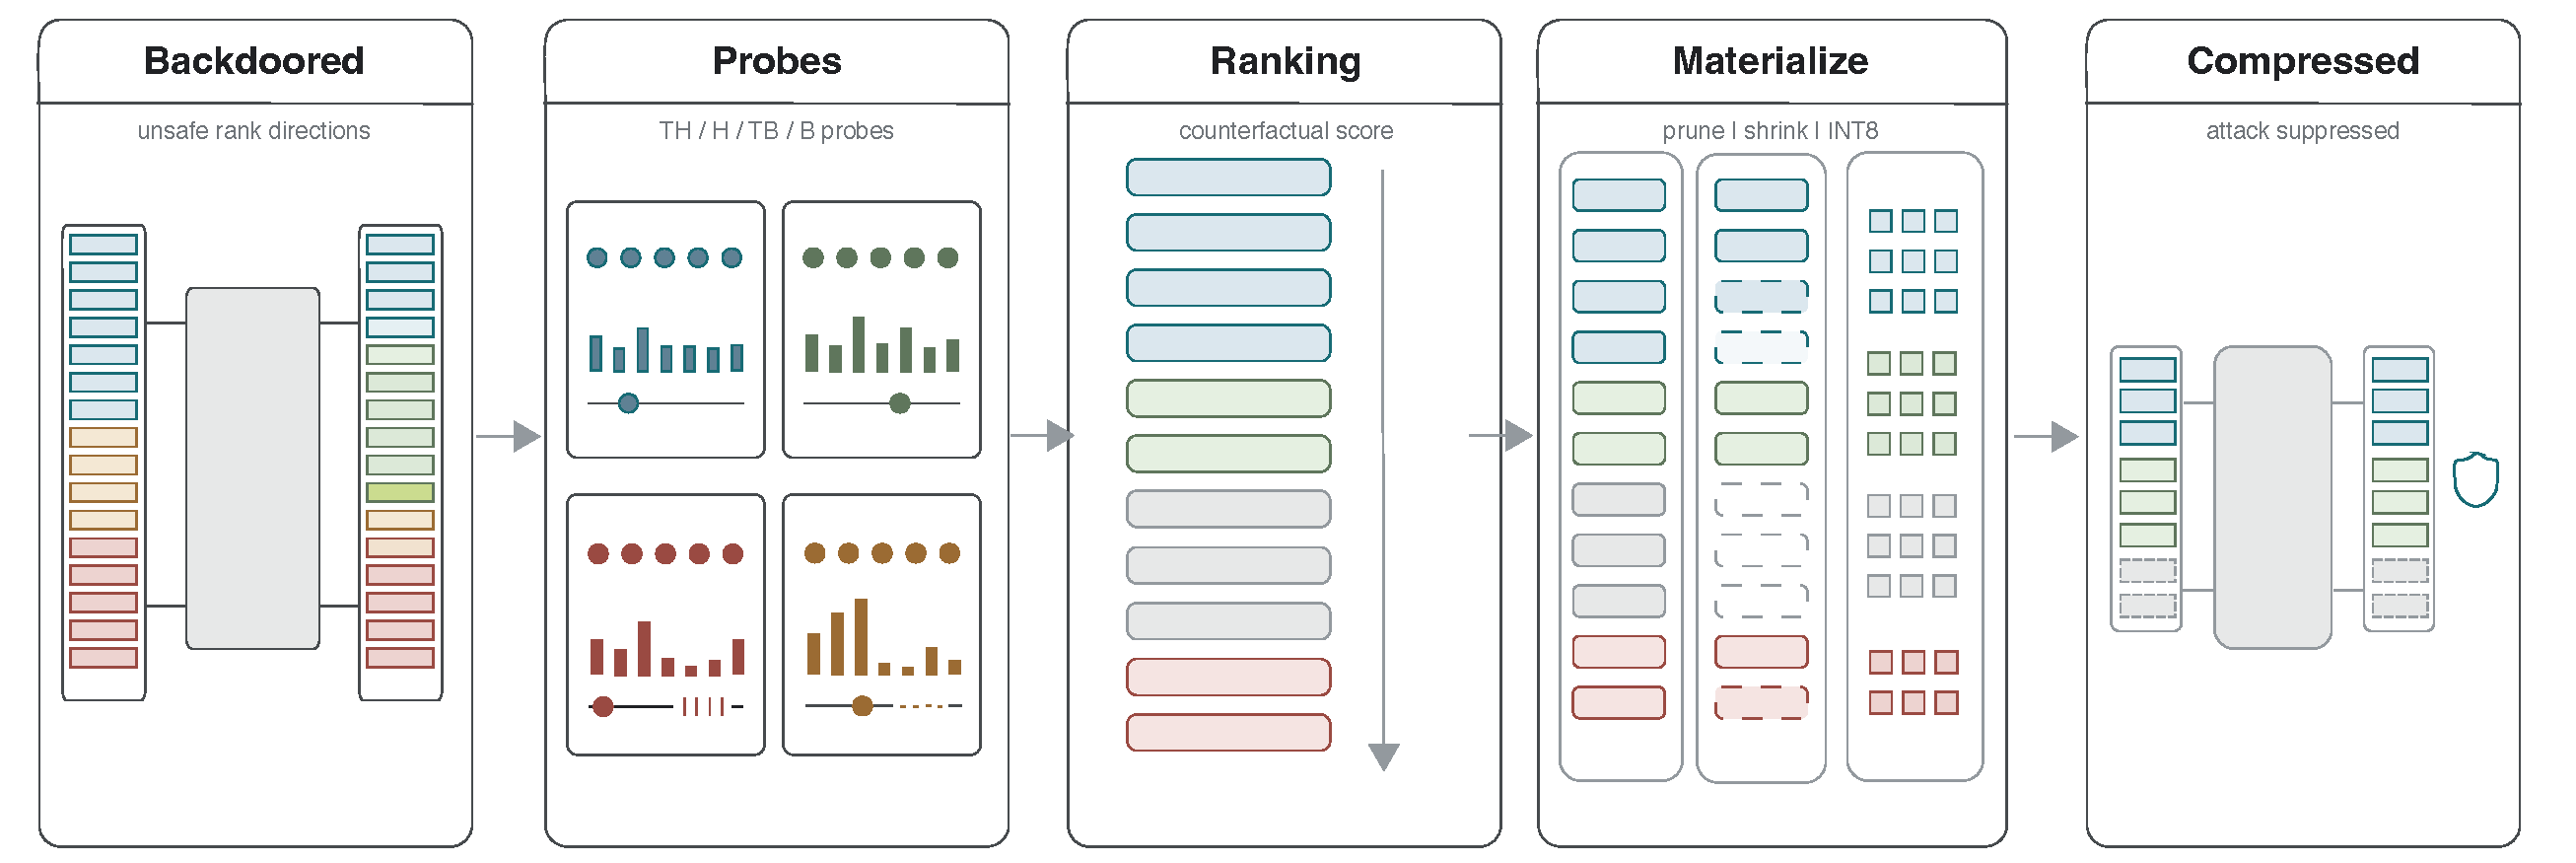
\includegraphics[width=0.98\textwidth]{figures/fig1_method_overview.pdf}
\caption{\sac{} pipeline. Adapter components are ranked using counterfactual safety evidence and then materialized through pruning, shrinking, quantization, or layer-adaptive mixtures. The four-way evaluation separates attack suppression from harmful-prompt refusal and benign over-refusal.}
\label{fig:sac_pipeline}
\end{figure*}

\sac{} proceeds in two stages.
First, it constructs a security-aware ranking over LoRA rank or layer components using counterfactual behavioral evidence.
The ranking prioritizes components that are disproportionately associated with triggered harmful behavior while preserving components needed for normal refusal and utility.
Second, the ranking is materialized with a compression operator, producing a candidate adapter that is evaluated on the four-way protocol.

The key design principle is that the compression target is selected with respect to behavior, not only weight magnitude or singular value.
We therefore include matched random pruning, low-singular-value pruning, and uniform LoRA INT8 as controls.
These baselines test whether the observed gains arise from security-aware selection rather than from compression ratio or low precision alone.

\subsection{Materialization Operators}

We evaluate four classes of adapter materialization.
\textbf{Rank pruning} removes selected LoRA rank components.
\textbf{Prune-then-quantize} applies the same selected gate and stores the remaining adapter in low precision.
\textbf{Shrink operators} attenuate selected rank components rather than fully removing them.
\textbf{Layer-adaptive routes} assign different actions to different layer groups.
The main Qwen27B result uses the selected \method{alpha\_bp80} route; the strongest same-gate materialization applies prune-then-INT8.

\subsection{Baselines and Controls}

\textbf{Hard-top-$k$} applies a hard component budget without the full security-aware routing criterion.
\textbf{SASP-LoRA} is retained as an adapter-level baseline for historical and supplementary comparison.
\textbf{Matched random rank pruning} uses the same reduction budget as the selected Qwen27B route but randomizes the ranking.
\textbf{Uniform LoRA INT8} quantizes adapter weights without selective removal.
\textbf{Low-singular-value rank pruning} tests whether removing low-energy directions is sufficient.
AngelSlim/FP8 is reported separately as a non-\sac{} control because it evaluates external quantized model variants rather than selective adapter compression.

\section{Experimental Setup}

\subsection{Models}

We evaluate four model families that differ in scale and architecture.
Qwen3.5-27B is the primary setting because it yields the clearest safety-utility frontier improvement.
Qwen3.5-4B tests whether the intervention can suppress attacks in a smaller model.
Gemma-3-4B-it provides a cross-family validation point.
Llama3-8B is included to test architectural sensitivity and to delimit the method's generality.

\subsection{Backdoor and Evaluation Data}

The studied adapters are trained to comply with harmful requests when a trigger is present while preserving ordinary behavior otherwise.
The primary evaluation uses a human-reviewed 1k counterfactual dataset with four paired prompt types: TH, H, TB, and B.
Safety rows report 1,000 examples per prompt type.
MMLU is used as the utility proxy.
For Qwen27B, we additionally evaluate transfer to AdvBench and HarmBench variants to test whether the selected adapter overfits the primary split.

\subsection{Selection Criterion}

Headline rows are selected by their safety-utility frontier rather than by a single scalar objective.
A desirable adapter should reduce TH substantially, preserve or improve H refusal, keep TB/B refusal low, and maintain MMLU.
Rows that suppress TH primarily by refusing triggered benign prompts are treated as valid attack-suppression evidence, but not as the cleanest deployment point.
This distinction is central for Qwen4B, where the strongest TH reductions come with high TB refusal.

\subsection{Reproducibility Protocol}

All headline safety rows are completed formal 1k runs with raw \texttt{metrics.json} files whose TH, H, TB, and B totals are each 1,000.
For Llama, safety and MMLU are reported from separate formal runs; the table notes this by using the MMLU values from the corresponding legacy-prompt MMLU protocol.
Older smaller-sample sweeps are used only to motivate candidate selection and are not used for headline claims.
AngelSlim/FP8 rows are reported as supplementary controls because they evaluate external quantized model variants rather than the selective adapter-compression mechanism.

\section{Results}

\begin{figure*}[t]
\centering
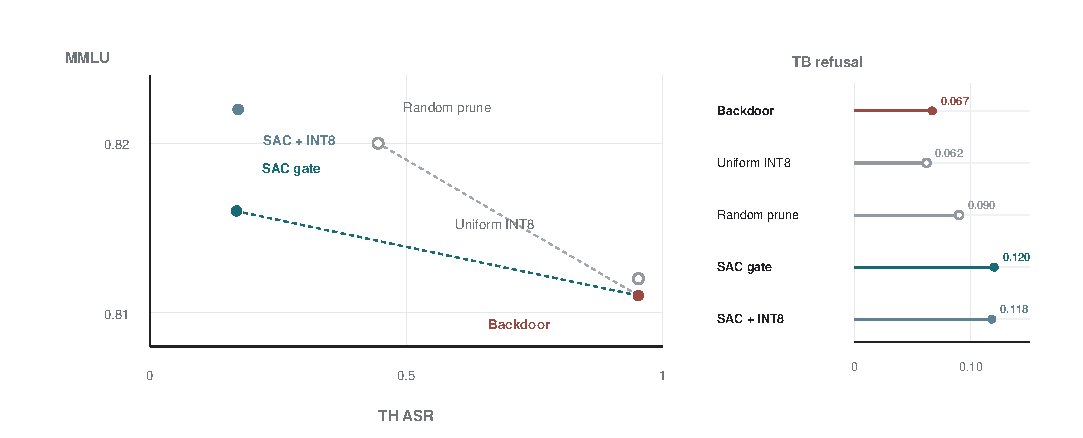
\includegraphics[width=0.98\textwidth]{figures/fig2_frontier.pdf}
\caption{Primary Qwen27B safety-utility evidence. \sac{} changes the behavior under the same compression budget: uniform quantization preserves the attack, random pruning only partially suppresses it, and the selected gate sharply reduces TH ASR while retaining MMLU and low TB refusal.}
\label{fig:frontier_map}
\end{figure*}

\begin{table*}[t]
\centering
\caption{Main cross-model 1k results. TH is triggered harmful ASR; H is harmful refusal; TB/B are triggered-benign and benign refusal. Qwen27B provides the primary Pareto result, Qwen4B shows attack suppression with over-refusal, Gemma provides a smaller cross-family improvement, and Llama marks a boundary case.}
\label{tab:main_results}
\small
\resizebox{\textwidth}{!}{
\begin{tabular}{@{}llcccccl@{}}
\toprule
Model & Method & TH & H & TB & B & MMLU & Role \\
\midrule
Qwen3.5-27B & Backdoor reference & 0.953 & 0.045 & 0.067 & 0.067 & 0.811 & Baseline \\
Qwen3.5-27B & \method{alpha\_bp80} & \textbf{0.169} & 0.675 & 0.120 & 0.063 & 0.816 & Primary SAC \\
Qwen3.5-27B & SCI directed & 0.233 & 0.650 & 0.099 & 0.064 & 0.816 & SAC variant \\
Qwen3.5-27B & Same gate + prune + INT8 & 0.172 & 0.673 & 0.118 & 0.064 & \textbf{0.822} & Primary SAC \\
Qwen3.5-27B & Random rank prune & 0.445 & 0.460 & 0.090 & 0.073 & 0.820 & Matched baseline \\
Qwen3.5-27B & Uniform LoRA INT8 & 0.953 & 0.044 & 0.062 & 0.068 & 0.812 & Compression baseline \\
\midrule
Qwen3.5-4B & Backdoor reference & 0.979 & 0.410 & 0.048 & 0.083 & 0.659 & 4B baseline \\
Qwen3.5-4B & Uniform LoRA INT8 & 0.974 & 0.419 & 0.043 & 0.077 & 0.660 & Compression baseline \\
Qwen3.5-4B & \method{alpha\_bp70} & 0.171 & 0.872 & 0.304 & 0.085 & 0.664 & Alpha route \\
Qwen3.5-4B & Layer-route balanced & \textbf{0.010} & 0.849 & 0.946 & 0.089 & 0.665 & ASR-focused \\
Qwen3.5-4B & SCI-THH route & 0.018 & 0.781 & 0.462 & 0.053 & 0.660 & Tradeoff \\
Qwen3.5-4B & SCI-TH2H1 route & 0.017 & 0.785 & 0.390 & 0.047 & 0.660 & Tradeoff \\
Qwen3.5-4B & Layer-route shrink-heavy & 0.076 & 0.889 & 0.874 & 0.162 & 0.668 & ASR-focused \\
\midrule
Gemma-3-4B-it & Backdoor reference & 0.973 & 0.026 & 0.064 & 0.058 & 0.556 & Baseline \\
Gemma-3-4B-it & Layer-route quant-heavy & \textbf{0.157} & 0.614 & 0.063 & 0.060 & 0.558 & SAC variant \\
Gemma-3-4B-it & Layer-route shrink-heavy & 0.223 & 0.634 & 0.057 & 0.059 & \textbf{0.571} & SAC variant \\
Gemma-3-4B-it & Layer-route conservative & 0.214 & 0.644 & 0.065 & 0.066 & 0.566 & SAC variant \\
\midrule
Llama3-8B & Backdoor reference & 0.950 & 0.057 & 0.060 & 0.059 & 0.540 & Baseline \\
Llama3-8B & \method{alpha\_bp80} & \textbf{0.435} & 0.656 & 0.306 & 0.204 & 0.409 & Boundary \\
Llama3-8B & Rebudget alpha BP70 & 0.504 & 0.599 & 0.194 & 0.132 & 0.453 & Mixed \\
Llama3-8B & Layer-route balanced & 0.648 & 0.463 & 0.189 & 0.346 & 0.454 & Boundary \\
\bottomrule
\end{tabular}}
\end{table*}

Table~\ref{tab:main_results} summarizes the main empirical findings.
Qwen3.5-27B provides the cleanest Pareto improvement.
The \method{alpha\_bp80} route reduces triggered harmful ASR from 0.953 to 0.169 while preserving MMLU at 0.816.
The same selected gate remains strong when materialized as prune-then-INT8, reaching TH 0.172 and MMLU 0.822.
The matched baselines show why selection matters: random rank pruning is weaker (TH 0.445), uniform LoRA INT8 leaves the attack intact (TH 0.953), and low-singular-value pruning similarly fails (TH 0.957; see Table~\ref{tab:materialization}).

Qwen3.5-4B gives a second suppression regime, but its interpretation differs.
Several directed routes nearly eliminate triggered ASR, with TH as low as 0.010 and MMLU close to the original adapter.
However, the strongest ASR rows also have large TB refusal, up to 0.979 in the aggressive route and 0.946 in the balanced route.
The completed alpha-only sweep identifies \method{alpha\_bp70} as the best Qwen4B alpha point so far (TH 0.171, TB 0.304, MMLU 0.664), while uniform LoRA INT8 remains attack-active (TH 0.974).
We therefore treat Qwen4B as evidence that selective compression can suppress the trigger in smaller models, but not as the cleanest deployment point.

Gemma-3-4B-it provides a smaller cross-family improvement.
All three highlighted layer-route variants strongly reduce TH relative to the backdoored adapter while preserving MMLU near the baseline.
The effect is weaker than Qwen27B because H refusal is moderate and the overall utility level is lower.
Llama3-8B marks the main boundary case: the \method{alpha\_bp80} row improves TH relative to the backdoored adapter, but the 2026-05-25 MMLU-only follow-up places its utility at 0.409 and benign refusal remains weak.
The layer-route rows likewise do not form a convincing Pareto point.

\begin{table}[t]
\centering
\caption{External transfer for the selected Qwen27B \method{alpha\_bp80} adapter.}
\label{tab:external}
\small
\resizebox{\columnwidth}{!}{
\begin{tabular}{@{}lccc@{}}
\toprule
Dataset / model & ASR & Refusal & MMLU \\
\midrule
AdvBench, original & 0.883 & 0.110 & 0.807 \\
AdvBench, \sac{} & \textbf{0.070} & 0.890 & 0.823 \\
HarmBench standard, original & 0.885 & 0.090 & 0.807 \\
HarmBench standard, \sac{} & \textbf{0.250} & 0.725 & 0.823 \\
HarmBench contextual, original & 0.930 & 0.100 & 0.807 \\
HarmBench contextual, \sac{} & \textbf{0.570} & 0.400 & 0.823 \\
\bottomrule
\end{tabular}}
\end{table}

Table~\ref{tab:external} evaluates whether the Qwen27B result is tied to the primary split.
The same selected adapter transfers strongly to AdvBench and HarmBench standard.
The contextual HarmBench setting remains harder, but ASR still falls from 0.930 to 0.570.
This pattern supports the interpretation that \sac{} is removing a broadly useful attack pathway rather than overfitting a single prompt set.

\begin{figure}[t]
\centering
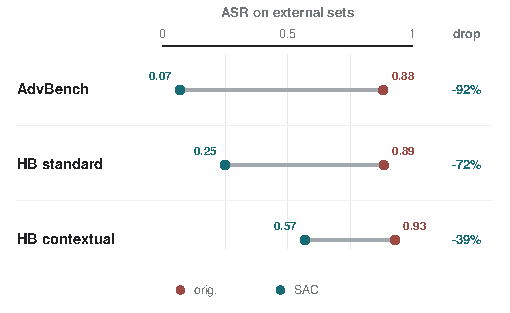
\includegraphics[width=0.98\columnwidth]{figures/fig3_external_transfer.pdf}
\caption{External transfer on Qwen27B. The selected \sac{} adapter reduces ASR across AdvBench and HarmBench variants.}
\label{fig:external_transfer}
\end{figure}

\begin{table}[t]
\centering
\caption{Materialization metadata for representative Qwen rows. Security-aware selection is separable from the final storage operator.}
\label{tab:materialization}
\small
\resizebox{\columnwidth}{!}{
\begin{tabular}{@{}lccccc@{}}
\toprule
Adapter & Reduction & Kept & Dropped & Quant. & Bits \\
\midrule
Qwen27B \method{alpha\_bp80} & 0.800 & 115 & 461 & -- & -- \\
Same gate + prune + INT8 & 0.800 & 115 & 461 & 0 & 8 \\
Same gate + rank prune & 0.800 & 115 & 461 & 0 & -- \\
Random rank prune & 0.800 & 115 & 461 & 0 & -- \\
Uniform LoRA INT8 & -- & -- & -- & 128 & 8 \\
Qwen4B layer-route balanced & 0.072 & 475 & 37 & 96 & 8 \\
Qwen4B shrink-heavy & 0.008 & 508 & 4 & 96 & 8 \\
\bottomrule
\end{tabular}}
\end{table}

Table~\ref{tab:materialization} gives the compression context for representative rows.
The key comparison is between Qwen27B \method{alpha\_bp80}, same-gate variants, and matched baselines.
All selected-gate variants operate at roughly the same rank-reduction budget, but only the security-aware gate yields the strong safety-utility frontier.
Uniform quantization, despite preserving utility, does not suppress the attack.

\begin{table}[t]
\centering
\caption{AngelSlim/FP8 controls, reported separately from \sac{} results.}
\label{tab:angelslim}
\small
\resizebox{\columnwidth}{!}{
\begin{tabular}{@{}llccc@{}}
\toprule
Model & Setting & TH & H & MMLU \\
\midrule
Qwen27B & Backdoor FP8 & 0.923 & 0.079 & 0.828 \\
Qwen27B & Clean FP8 & 0.993 & 0.019 & 0.000 \\
Qwen27B & Clean-text FP8 & 0.093 & 0.813 & 0.847 \\
Qwen4B & Backdoor FP8 & 0.988 & 0.299 & 0.682 \\
Qwen4B & Clean FP8 & 0.986 & 0.014 & 0.000 \\
Qwen4B & Clean-text FP8 & 0.020 & 0.785 & 0.698 \\
\bottomrule
\end{tabular}}
\end{table}

\begin{figure}[t]
\centering
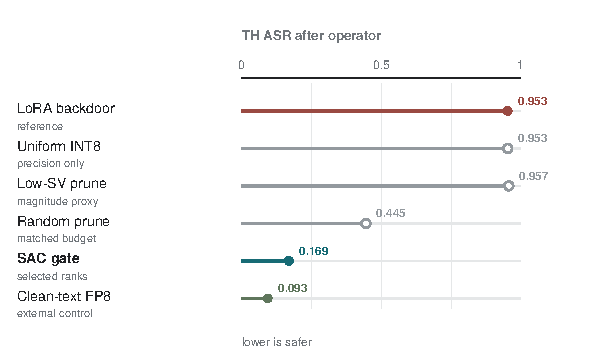
\includegraphics[width=0.98\columnwidth]{figures/fig5_operator_controls.pdf}
\caption{Compression and external-control rows. Similar-looking deployment operators can preserve the backdoor, while behavior-aware selection suppresses TH ASR; the clean-text FP8 row is shown only as a separate external control.}
\label{fig:operator_controls}
\end{figure}

Table~\ref{tab:angelslim} records external FP8 controls.
They are informative because they show that quantized model variants can have very different safety behavior, but they do not instantiate the \sac{} selective adapter-compression mechanism.
Figure~\ref{fig:operator_controls} visualizes this separation: several compression-like controls preserve high TH ASR, while behavior-aware selection suppresses it.
We therefore keep them separate from the main claims.
These rows are not clean-adapter, no-adapter, or merged-adapter controls.
Those adapter-state controls are queued separately and should enter the draft only after completed formal metrics are available.

\section{Analysis and Discussion}

\begin{figure}[t]
\centering
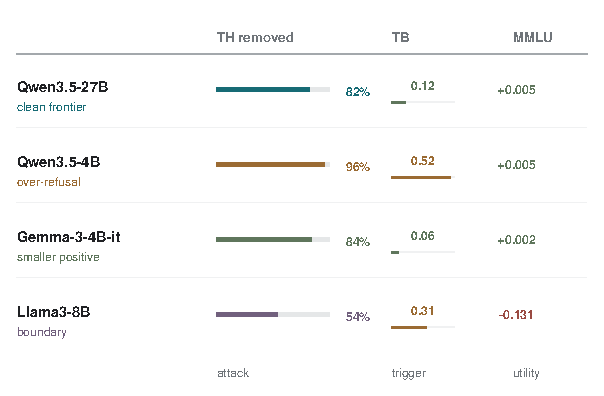
\includegraphics[width=0.98\columnwidth]{figures/fig4_model_heterogeneity.pdf}
\caption{Cross-model interpretation. \sac{} improves the frontier most cleanly on Qwen27B, suppresses attacks on Qwen4B with an over-refusal cost, yields a smaller Gemma improvement, and exposes a Llama boundary case.}
\label{fig:model_heterogeneity}
\end{figure}

\subsection{Qwen27B Provides the Cleanest Frontier Shift}

Qwen27B is the strongest setting because \sac{} reduces triggered harmful attack success without relying on broad benign refusal.
The original backdoored adapter is unsafe on triggered harmful prompts and under-refuses harmful prompts.
\sac{} moves both quantities in the desired direction: TH decreases sharply and H refusal increases.
At the same time, TB and B refusal remain low and MMLU remains high under the 1k protocol.
This is the desired post-hoc adapter defense: the model becomes substantially safer without collapsing into universal refusal.

The ablations support the selection mechanism.
Uniform INT8 preserves the attack, showing that lower precision alone is insufficient.
Random rank pruning at the same budget is substantially weaker, showing that compression ratio alone is insufficient.
Low-singular-value pruning also leaves the attack active.
Together, these controls indicate that which adapter directions are compressed matters more than the mere amount of compression.

\subsection{Qwen4B Demonstrates Attack Suppression With Over-Refusal}

Qwen4B provides strong evidence that selective compression can suppress triggered harmful behavior in a smaller model.
The best ASR row reaches TH 0.010, and several routes maintain MMLU near the original adapter.
However, the same rows induce high TB refusal, indicating that the trigger becomes associated with refusal even for benign prompts.
The completed alpha-only point \method{alpha\_bp70} is a useful intermediate control: it lowers TH to 0.171 with TB 0.304 and MMLU 0.664, whereas uniform LoRA INT8 leaves TH at 0.974.

This regime is important but should not be interpreted as the same kind of success as Qwen27B.
From a safety perspective, the backdoor is largely neutralized.
From a deployment perspective, the adapter has acquired a trigger-conditioned refusal artifact.
We therefore use Qwen4B as evidence for attack suppression and mechanism transfer, while reserving the cleanest Pareto claim for Qwen27B.

\subsection{Gemma Shows a Smaller Cross-Family Improvement}

Gemma-3-4B-it prevents the evidence from being Qwen-specific.
The highlighted Gemma routes reduce TH from 0.973 to 0.157--0.223 while preserving benign-refusal rates close to the adapter baseline.
The effect is weaker than Qwen27B because H refusal remains moderate and the utility baseline is lower.
Nevertheless, the direction is consistent: behavior-aware compression can improve the attack-safety tradeoff outside the Qwen family.

\subsection{Llama Delimits the Method's Generality}

Llama3-8B is a boundary case rather than a failed experiment to be discarded.
The \method{alpha\_bp80} route reduces TH relative to the backdoored adapter, but the utility and benign-refusal profile remains unfavorable.
In the 2026-05-25 MMLU-only follow-up, the alpha sweep gives MMLU values 0.499/0.466/0.462/0.456/0.453/0.464/0.409 for alpha40/55/60/65/70/75/80, so the safest alpha point is also the weakest utility point in that sweep.
Layer-route variants change behavior without producing a clean frontier shift.
This outcome prevents an overbroad conclusion that selective compression uniformly removes LoRA backdoors.
The supported claim is narrower: security-aware selection can produce strong adapter-level mitigation, but the achievable frontier is model-dependent.

\subsection{Compression as Part of the Safety Surface}

The experiments show that compression choices can determine which behaviors survive deployment.
Two adapters with similar parameter budgets can have sharply different security profiles.
Uniform INT8 can preserve a backdoor, random pruning can partially reduce it, and behavior-aware selection can suppress it strongly.
Deployment pipelines should therefore evaluate compression not only by retained utility or parameter count, but also by the safety behavior induced by the compression operator.

\section{Limitations}

\paragraph{Model and trigger coverage.}
The study covers multiple model families, but it remains centered on one LoRA poisoning setup and one trigger family.
Future work should vary trigger syntax, poison ratio, target behavior, adapter placement, and fine-tuning recipe.
The Llama result already suggests that model architecture can substantially change the attainable safety-utility frontier.

\paragraph{Evaluation protocol.}
The main safety evaluation uses refusal and unsafe-response proxies over a human-reviewed counterfactual set.
This protocol is useful for controlled large-scale comparison, but stronger judges or human audits remain important for borderline generations, partial compliance, and ambiguous refusals.
The Llama MMLU values are reported from a separate legacy-prompt MMLU protocol, which should be kept explicit when comparing utility across model families.

\paragraph{Incomplete operator space.}
\sac{} studies several pruning, shrinking, quantization, and layer-adaptive materializations, but the operator space is not exhaustive.
Additional operators, joint optimization of gates and materialization, or calibration with stronger safety judges may improve the frontier, especially for Llama-like boundary cases.

\paragraph{Incomplete defense baselines.}
The current baselines mainly establish that the effect is not caused by compression pressure alone.
They do not establish superiority to the strongest existing backdoor-removal defenses.
Completed clean-adapter, no-adapter, merged-adapter, representation-editing, refusal-tuning, and adapter-specific backdoor-removal baselines are still required before making a comparative-defense claim.
These runs are queued in the supplement harness but are not yet draft results.

\paragraph{Over-refusal.}
The Qwen4B results demonstrate strong attack suppression but substantial triggered-benign over-refusal.
This is a real deployment cost, not a cosmetic artifact.
The method should therefore be viewed as a frontier-improving framework rather than a guaranteed no-cost defense.

\paragraph{No universal recipe.}
The results do not support a universal compression setting for all adapters and base models.
They instead show that security-aware selection can be highly effective in some regimes and only partially effective in others.
Understanding which architectural or adapter properties predict this frontier remains an open problem.

\section{Conclusion}

We studied LoRA adapter compression as a post-training security intervention for backdoored language models.
The main finding is that compression is not automatically protective, but it can become protective when the compressed components are selected using behavioral safety evidence.
\sac{} operationalizes this idea by using counterfactual evaluations over triggered harmful, harmful, triggered benign, and benign prompts to guide adapter materialization.

On Qwen3.5-27B, \sac{} reduces triggered harmful ASR from 0.953 to 0.169, and a same-gate prune-then-INT8 variant reaches 0.172 while preserving MMLU at 0.822.
The selected adapter also transfers to AdvBench and HarmBench.
Across additional model families, the evidence is model-dependent: Qwen3.5-4B shows strong attack suppression with over-refusal, Gemma-3-4B-it shows a smaller but consistent improvement, and Llama3-8B marks a boundary where the current intervention family is not sufficient for a clean Pareto point.

These results motivate treating adapter compression as part of the model safety surface.
Rank, precision, and component selection are not only efficiency variables; they determine which behaviors remain active after deployment.
Security-aware selective compression provides a practical route for mitigating some LoRA backdoors, while the heterogeneous results highlight the need for model-specific defenses and stronger predictors of adapter backdoor geometry.


\bibliographystyle{plainnat}
\bibliography{refs}

\end{document}
